\chapter{計測用プログラムの概要}
\label{cha:program}

本章では、本研究において作成した 4 種類のスクリプト言語の実行時間を比較検討するためのプログラムについて述べる。 
本研究では、それぞれのスクリプト言語の基本的な実行時間を比較検討するためにバブルソート、フィボナッチ数列、
ライプニッツ級数による円周率の算出プログラムを作成した。これに加えて、Web サービスや Web アプリケーションで
頻繁に使用される正規表現の実行時間を比較検討するために、該当の機能を利用したプログラムも作成した。

\section{バブルソート}
\label{cha:program:sort}

まず始めに、数値配列のソートに関する実行時間を比較検討するために、バブルソートを行うプログラムを作成した。
バブルソートは、ソートアルゴリズムの一つで実行の速度が遅く実用的ではないが、仕組みが理解しやすいため初学者の学習によく利用されている。
このアルゴリズムは、ある数値配列における隣接する要素の大小比較および入れ替え操作を全ての要素に対して行う。
一回目の比較が終わると、対象とする数列の最大値が確定し、該当の右端に移動した状態になる。
二回目は、一回目の操作で確定した最大値を除いた数値配列に対して同様の操作を行う。
この操作を繰り返す事で対象となる数値配列のソートを行う。

バブルソートプログラムの計算量は O$(n^{2})$ となる。
これはソートアルゴリズムとしては計算量が多く、あまり実用的ではない。
例えば、クイックソートの計算量は O$(n\log{n})$ であり、バブルソートよりも計算量が少ない。
しかし、現在のコンピューターの性能では負荷の少ないクイックソートは、非常に短い時間で処理が終了してしまうため計測が難しいと考えた。
そのため本研究では、計算量が多く、スクリプト言語の差が顕著に出ることが予想されるバブルソートを比較検討対象プログラムとする事にした。

本研究において、Python で実装したプログラムを図~\ref{fig:b-rb} に示す。
このプログラムでは、テキストファイルから数値を読み取り、ソートした結果をテキストファイルに書き込む。
この図の 1 行目で関数 bsort() を定義しており、2 行目から 6 行目でアルゴリズムを実装している。
この図のその他の処理は、テキストファイルからソートする数値を読み込む処理である。

\section{フィボナッチ数列}
\label{cha:program:fibonacci}

次に、スクリプト言語の再起呼び出しに関する実行時間を比較検討をするために、フィボナッチ数列を算出するプログラムを作成した。
フィボナッチ数列とは「1, 1, 2, 3, 5, 8, 13, 21, 34, 55, 89, 144, ...」という様に、
数列のそれぞれの値が 1 つ前と 2 つ前の値の和になる数列である。
フィボナッチ数列は式~\ref{eq:fibonacci} で表す事ができる。

\begin{eqnarray}
\label{eq:fibonacci}
  F_{0}&=&0 \nonumber \\
  F_{1}&=&1 \\
  F_{n+1}&=&F_{n}+F_{n+1}(n≥0)\nonumber
\end{eqnarray}

この漸化式を再起呼び出しを用いて、プログラム上に実装する。

本研究において、Python で実装したものを 図~\ref{fig:f-py} に示す。
この図の 3 行目に定義した fib() 関数を 7 行目で再起呼び出しを行っている。
fib() の引数が 0 か 1 になるまで引数に指定される値を 1 ずつ減らしながら fib() を呼び出し続ける。

再起呼び出しを使ったプログラムは for 文などのループ処理に比べて、
関数呼び出し時の負荷が何度も存在するため実行時間が増加する傾向にある。
今回のプログラムも導出する数が 1 大きくなるごとに再起呼び出しの回数が指数関数的に増加する。
今回作成したプログラムの計算量は O$((\frac{1 +\sqrt{5}}{2})^{n-1})$ となる。
このような時間のかかる漸化式を使った実装は避けられており実用的ではなく、
一般的には、プログラミング言語の機能の一つであるメモ化などを使って実装することが多い。
しかし、本研究では再起呼び出しに関する処理能力を計測することを目的としていたため、効率の悪い漸化式での実装を行った。

\section{ライプニッツ級数による円周率の算出}
\label{cha:program:leibniz}

本節では、スクリプト言語の実行速度を比較検討するための、円周率を求めるプログラムについて説明する。
本研究では、円周率を求めるためにライプニッツ級数を用いた実装を行った。
ライプニッツ級数は、式~\ref{eq:leibniz} で表せる。

\begin{eqnarray} \label{eq:leibniz}
\sum_{n=0}^{\infty}\frac{(-1)^n}{2n+1}=\frac{\pi}{4}
\end{eqnarray}

この式を展開すると式~\ref{eq:leibniz2} のように表す事ができる。

\begin{eqnarray} \label{eq:leibniz2}
1-\frac{1}{3}+\frac{1}{5}-\frac{1}{7}+\cdots=\frac{\pi}{4}
\end{eqnarray}

ライプニッツ級数においては、実行回数を増やすと導出される円周率の精度が向上する。
例えば、10 億回実行すると円周率が 10 桁まで正しく導出される。
ライプニッツ級数は円周率の計算方法の中では収束が遅く効率も悪いが、
現在のコンピューターでその他の方法を使うと非常に早く収束してしまい、実行時間の計測が難しい。
したがって、ライプニッツ級数はプログラミング言語の実行速度を計測するのに適していると予想される。

本研究において、Python で実装したものを図~\ref{fig:p-py} に示す。
この図の 6 行目から 9 行目で、式~\ref{eq:leibniz} の左辺にあたるものを実装している。
また、10 行目で左辺を 4 倍することで円周率を求めている。
次に、PHP で実装したものを図~\ref{fig:p-php} に示す。
この図の 2 行目から 11 行目で同様の実装をしており、その他の部分は導出した解をテキストファイルに書き込む処理である。
この二つの図を比べると、ライプニッツ級数の実装方法にはほぼ差異がないことがわかる。
本研究では、残りの 2 つのスクリプト言語での実装に関しても同様に、計算量が同じになるように注意して実装している。
これらのプログラムの計算量は O(n) となり、実行時間は実行回数に比例する。

\section{正規表現}
\label{cha:program:regex}

最後に、スクリプト言語の正規表現に関する処理能力を比較検討するために、指定された文字列が URL かどうかを判別するプログラムを作成した。
このプログラムでは、URL の混在した任意の行数の文字列が記載されているテキストファイルを開き、その内容から正規表現を用いて URL を抽出し、出力する。

本研究において、Python で実装したものを図~\ref{fig:s-py} に示す。
この図を見ると、正規表現を扱うライブラリである "re" をインポートして関数 re.findall を使用している事が分かる。
次に、PHP で実装したものを図~\ref{fig:s-php} に示す。
この図を見ると、PHP では preg-match 関数が用いられている事が分かる。。
これらの関数は結果としては同じ振る舞いをするが、スクリプト言語ごとに実行速度が異なる結果になる事が予想される。

\begin{figure}[tb]
    \centering
    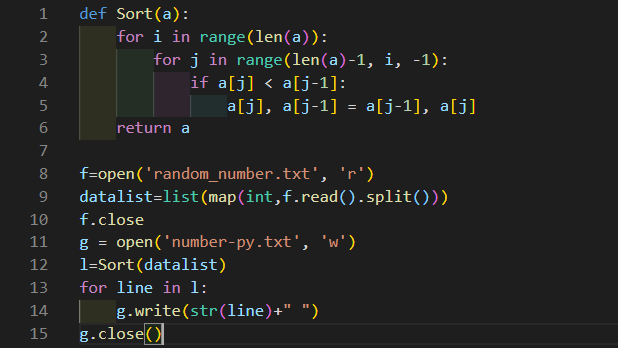
\includegraphics[width=13.5cm,keepaspectratio]{figure/b-rb.PNG}
    \caption{Python3 バブルソート}
    \label{fig:b-rb}
\end{figure}

\begin{figure}[tb]
    \centering
    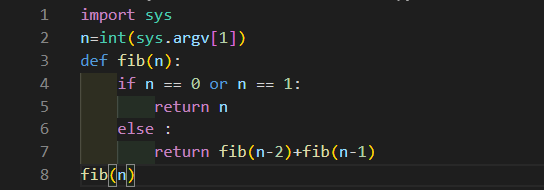
\includegraphics[width=13.5cm,keepaspectratio]{figure/f-py.PNG}
    \caption{Python3 フィボナッチ数列}
    \label{fig:f-py}
\end{figure}

\begin{figure}[tb]
    \centering
    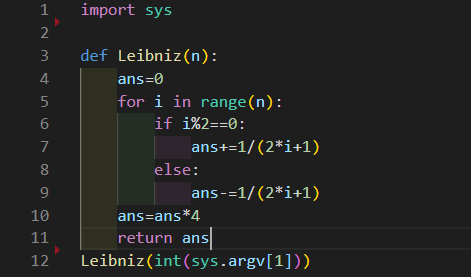
\includegraphics[width=13.5cm,keepaspectratio]{figure/p-py.PNG}
    \caption{Python3 円周率の算出}
    \label{fig:p-py}
\end{figure}

\begin{figure}[tb]
    \centering
    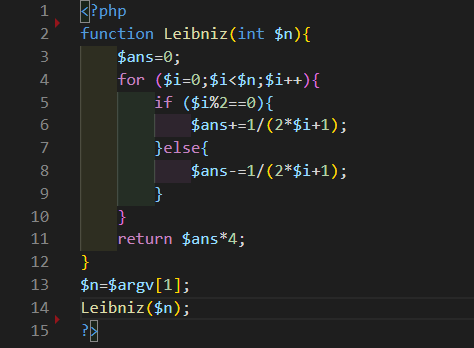
\includegraphics[width=13.5cm,keepaspectratio]{figure/p-php.PNG}
    \caption{PHP 円周率の算出}
    \label{fig:p-php}
\end{figure}
\begin{figure}[tb]
    \centering
        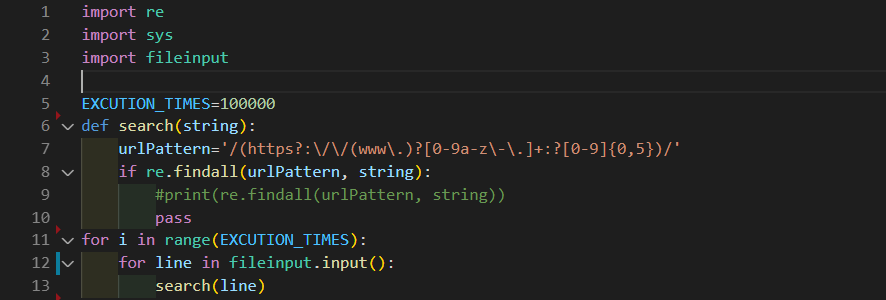
\includegraphics[width=13.5cm,keepaspectratio]{figure/s-py.PNG}
        \caption{Python3 正規表現}
        \label{fig:s-py}
\end{figure}

\begin{figure}[tb]
    \centering
        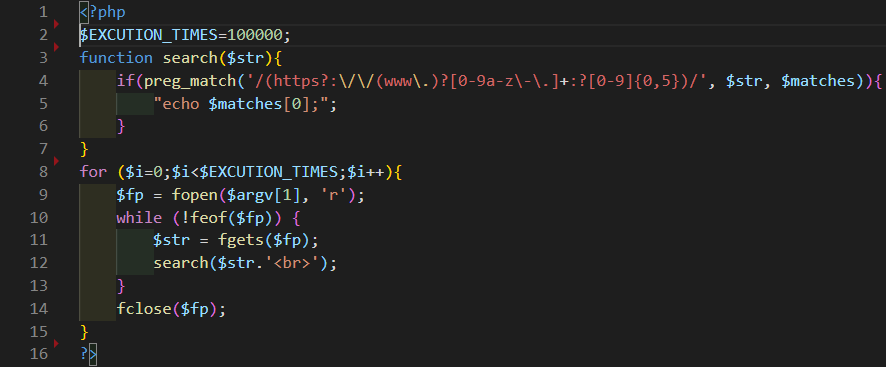
\includegraphics[width=13.5cm,keepaspectratio]{figure/s-php.PNG}
        \caption{PHP 正規表現}
        \label{fig:s-php}
\end{figure}
